\documentclass[12pt, a4paper]{article}
\usepackage[utf8]{inputenc}
\usepackage[polish]{babel}
\usepackage[T1]{fontenc}%polskie znaki
\usepackage[utf8]{inputenc}%polskie znaki

\usepackage{sectsty}
\usepackage{graphicx}
\usepackage{float}
\usepackage[hidelinks]{hyperref}

\newcommand{\subsubsubsection}[1]{\paragraph{#1}\mbox{}\\}
\setcounter{secnumdepth}{4}
\setcounter{tocdepth}{4}

% Margins
\topmargin=-0.45in
\evensidemargin=0in 
\oddsidemargin=0in
\textwidth=6.5in
\textheight=9.0in
\headsep=0.25in

\title{ Instrukcja korzystania z~serwisu TER}
\author{ Leszek Błażewski\\\\Damian Koper\\\\Karol Noga\\\\Michał Nawrot\\\\Mateusz Wojciechowski}
%\date{\today}

\begin{document}
\maketitle
\pagebreak

% Optional TOC
\tableofcontents
\pagebreak

%--Paper--

\section{Opis i~dostępna funkcjonalność narzędzia}

Narzędzie \textit{TER} (z ang. text entities relations) powstało w~celu umożliwienia czytelnego zaprezentowania wyników usługi \textit{NER} (z ang. named entity recognition), która pozwala na~rozpoznawanie nazw własnych i~wyrażeń temporalnych w~zadanych przez użytkownika tekstach. Opisywane narzędzie rozszerza serwis NER, między innymi poprzez odpowiednie wyliczanie relacji pomiędzy odnalezionymi bytami, na~podstawie zadanych wcześniej przez użytkownika parametrów, prezentację obliczonych relacji w formie modyfikowalnego grafu, zapisanie pracy do pliku, umożliwiając jej wznowienie na~innym urządzeniu oraz~eksport wyników do~kilku popularnych formatów.

\section{Instrukcja użytkowania}

W~poniższym dokumencie opisano wszystkie dostępne funkcjonalności zrealizowanego systemu wraz z~realnym przykładem, gdzie pokazano ich wykorzystanie, tak aby czytelnik zrozumiał działanie poszczególnych opcji i~potrafił otrzymać pożądany rezultat. Do dokumentu załączono również dwa pliki, dzięki którym można śledzić wszystkie prezentowane operacje na bieżąco i~wraz z~instrukcją przetestować działanie odpowiednich mechanizmów.

\pagebreak

\subsection{Startowy widok aplikacji}

\begin{figure}[H]
  \centering
  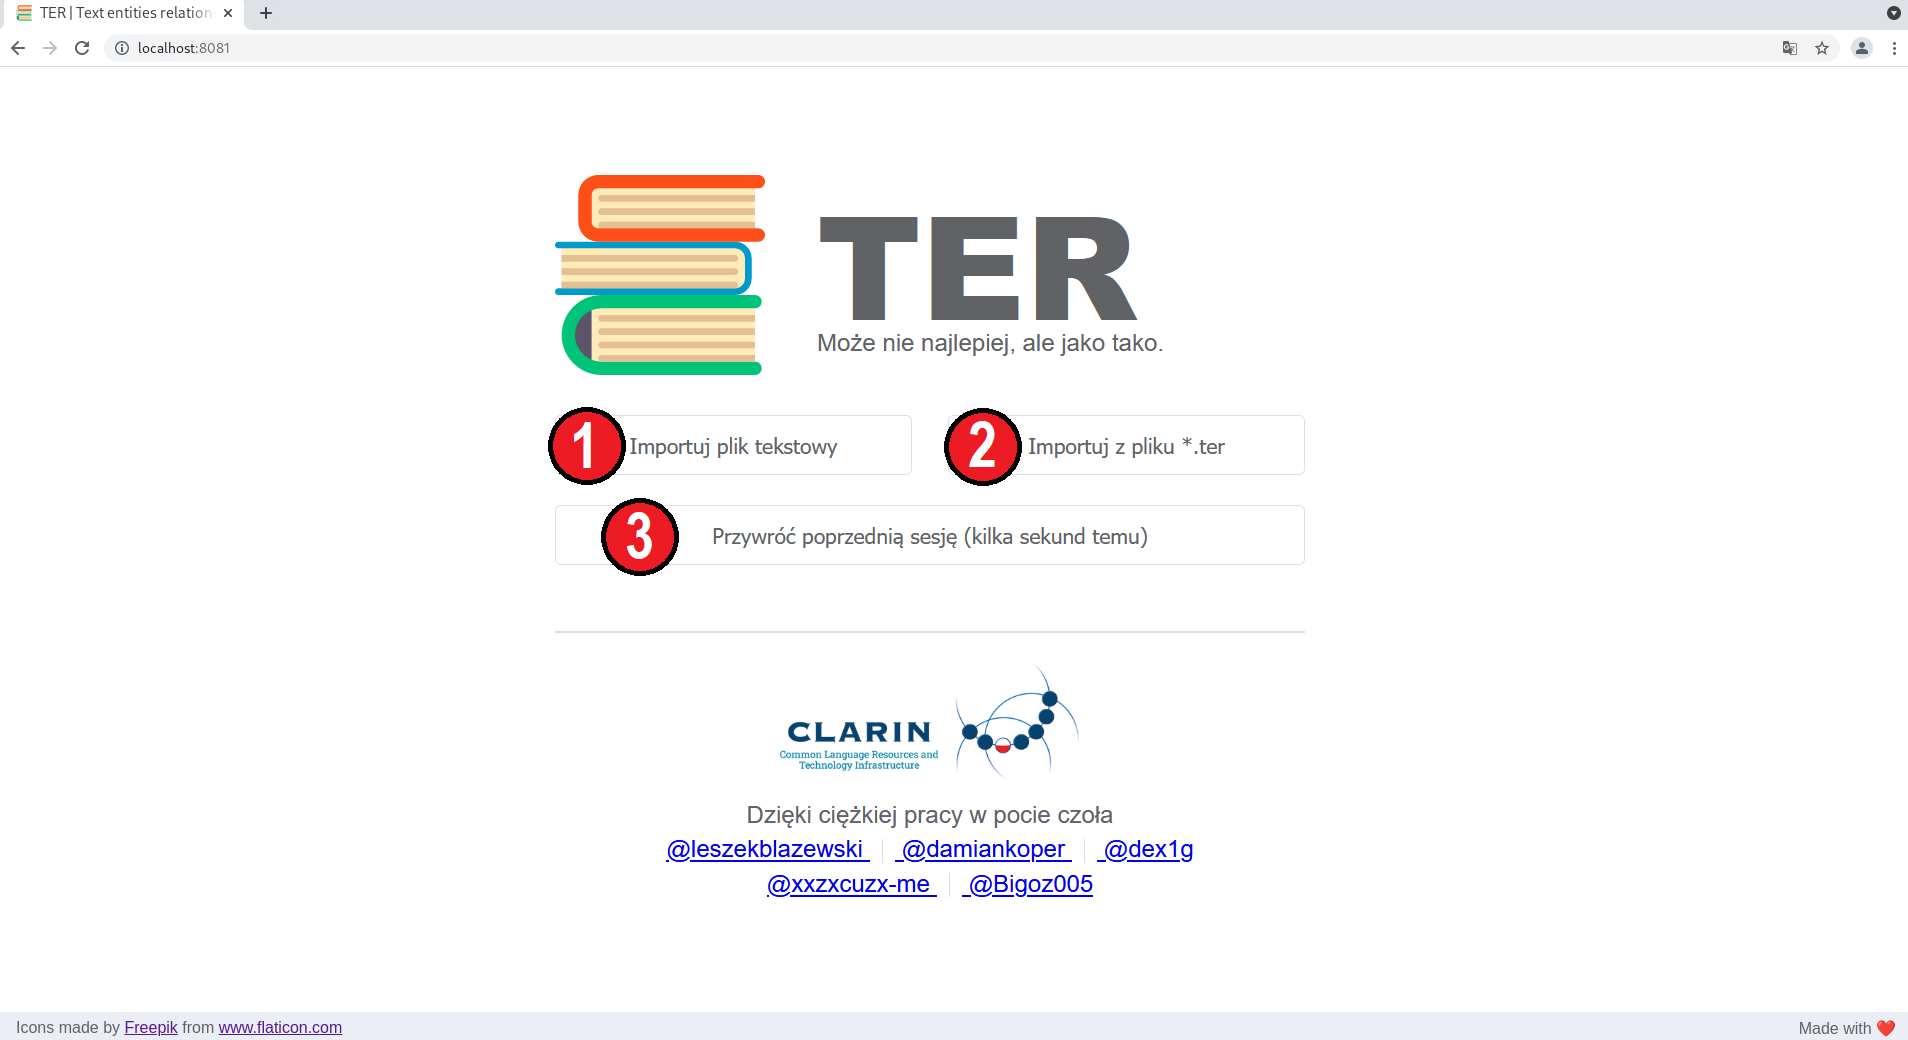
\includegraphics[width=\linewidth]{images/homepage.png}
  \caption{Widok startowy}
  \label{main-view}
\end{figure}

\textbf{Opcja 1, import z~pliku} -- Naciskamy przycisk, jeśli chcemy wczytać własny tekst z~pliku i~poddać go analizie.\\

\noindent\textbf{Opcja 2, import z~pliku ter} -- Wybieramy opcję, jeśli posiadamy wygenerowany wcześniej przez aplikację plik o rozszerzeniu \textit{*.ter} lub otrzymaliśmy go od innej osoby. Opcja ta pomija etap analizy tekstu i~pozwala bezpośrednio przejść do widoku grafu, który reprezentuje stan zapisany wcześniej podczas innej sesji w~aplikacji. Praca z~widokiem grafu została opisana w~sekcji \ref{section:graph}.\\

\noindent\textbf{Opcja 3, przewrócenie sesji} -- Jeśli pracowaliśmy już z~aplikacją i~poddaliśmy jakiś tekst analizie, nasz wcześniej uzyskany stan danych został zapisany i~poprzez naciśnięcie przycisku możemy kontynuować pracę od tamtego momentu, przechodząc bezpośrednio na widok grafu. \textit{Uwaga} funkcja ta dostępna jest w~zakresie instancji przeglądarki, oznacza to przykładowo, że pracując na przeglądarce Firefox a~następnie próbując przywrócić stan w~przeglądarce Chrome, zobaczymy, że przycisk będzie niedostępny. Używanie trybu prywatnego/incognito lub czyszczenie danych historii przeglądania również uniemożliwia przywrócenie ostatniego stanu. Praca z~widokiem grafu została opisana w~sekcji \ref{section:graph}.

\pagebreak

\subsection{Widok importu plików}

W tej sekcji konfigurujemy wszystkie parametry, które konieczne są podczas analizy importowanego tekstu oraz wykorzystywane są do identyfikacji i~modyfikacji relacji pomiędzy odnalezionymi w~tekście bytami.

W instrukcji poddamy analizie dostępne publicznie opowiadanie Władysława Szlengela pod tytułem \textit{Co czytałem umarłym}. Plik z~opowiadaniem został dołączony do instrukcji, tak aby każdy mógł na bieżąco podążać z~zawartymi instrukcjami.

\subsubsection{Dane wejściowe}

\begin{figure}[H]
  \centering
  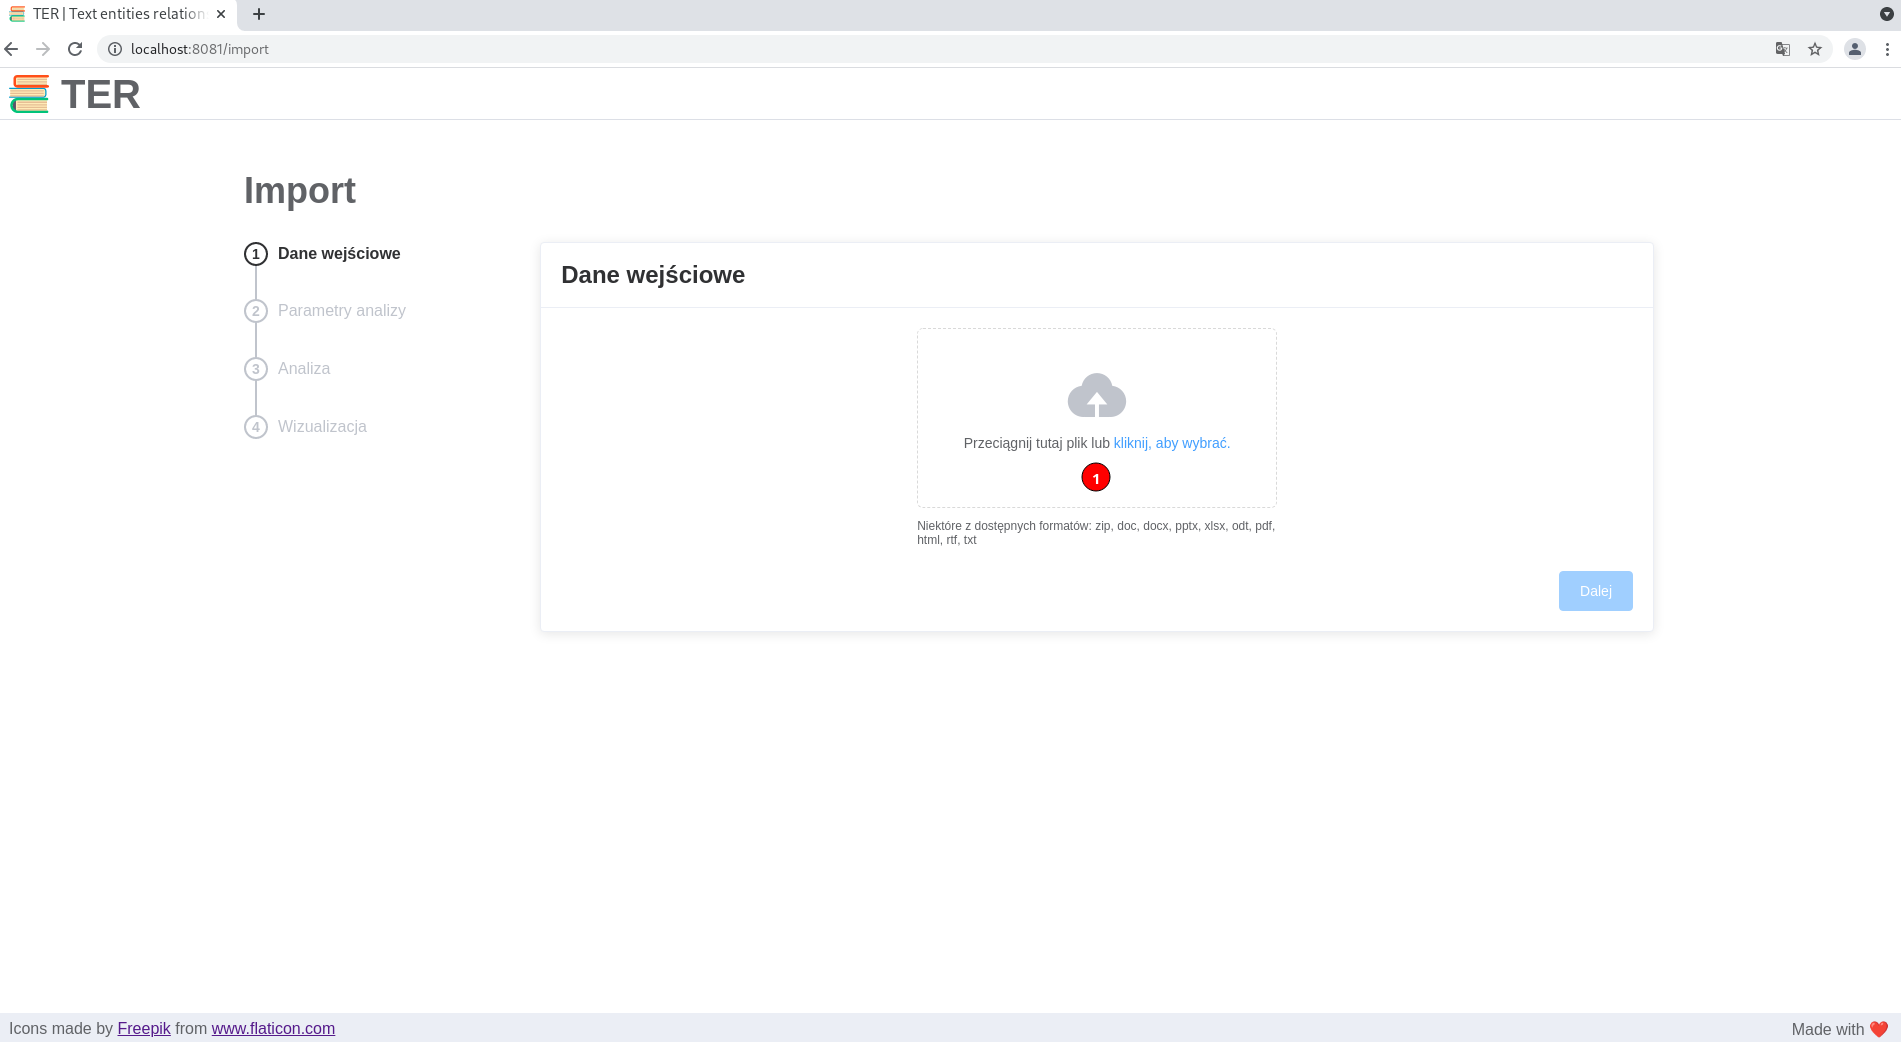
\includegraphics[width=\linewidth]{images/import-before-file.png}
  \caption{Importowanie pliku}
\end{figure}

Po naciśnięciu w~zadane miejsce ukaże nam się okno systemowe, gdzie wybieramy plik z~tekstem, który następnie poddany zostanie analizie. Plik można również przeciągnąć w~wyznaczoną strefę. Jeśli spróbujemy załączyć dwa pliki ukaże nam się następujący komunikat.

\begin{figure}[H]
  \centering
  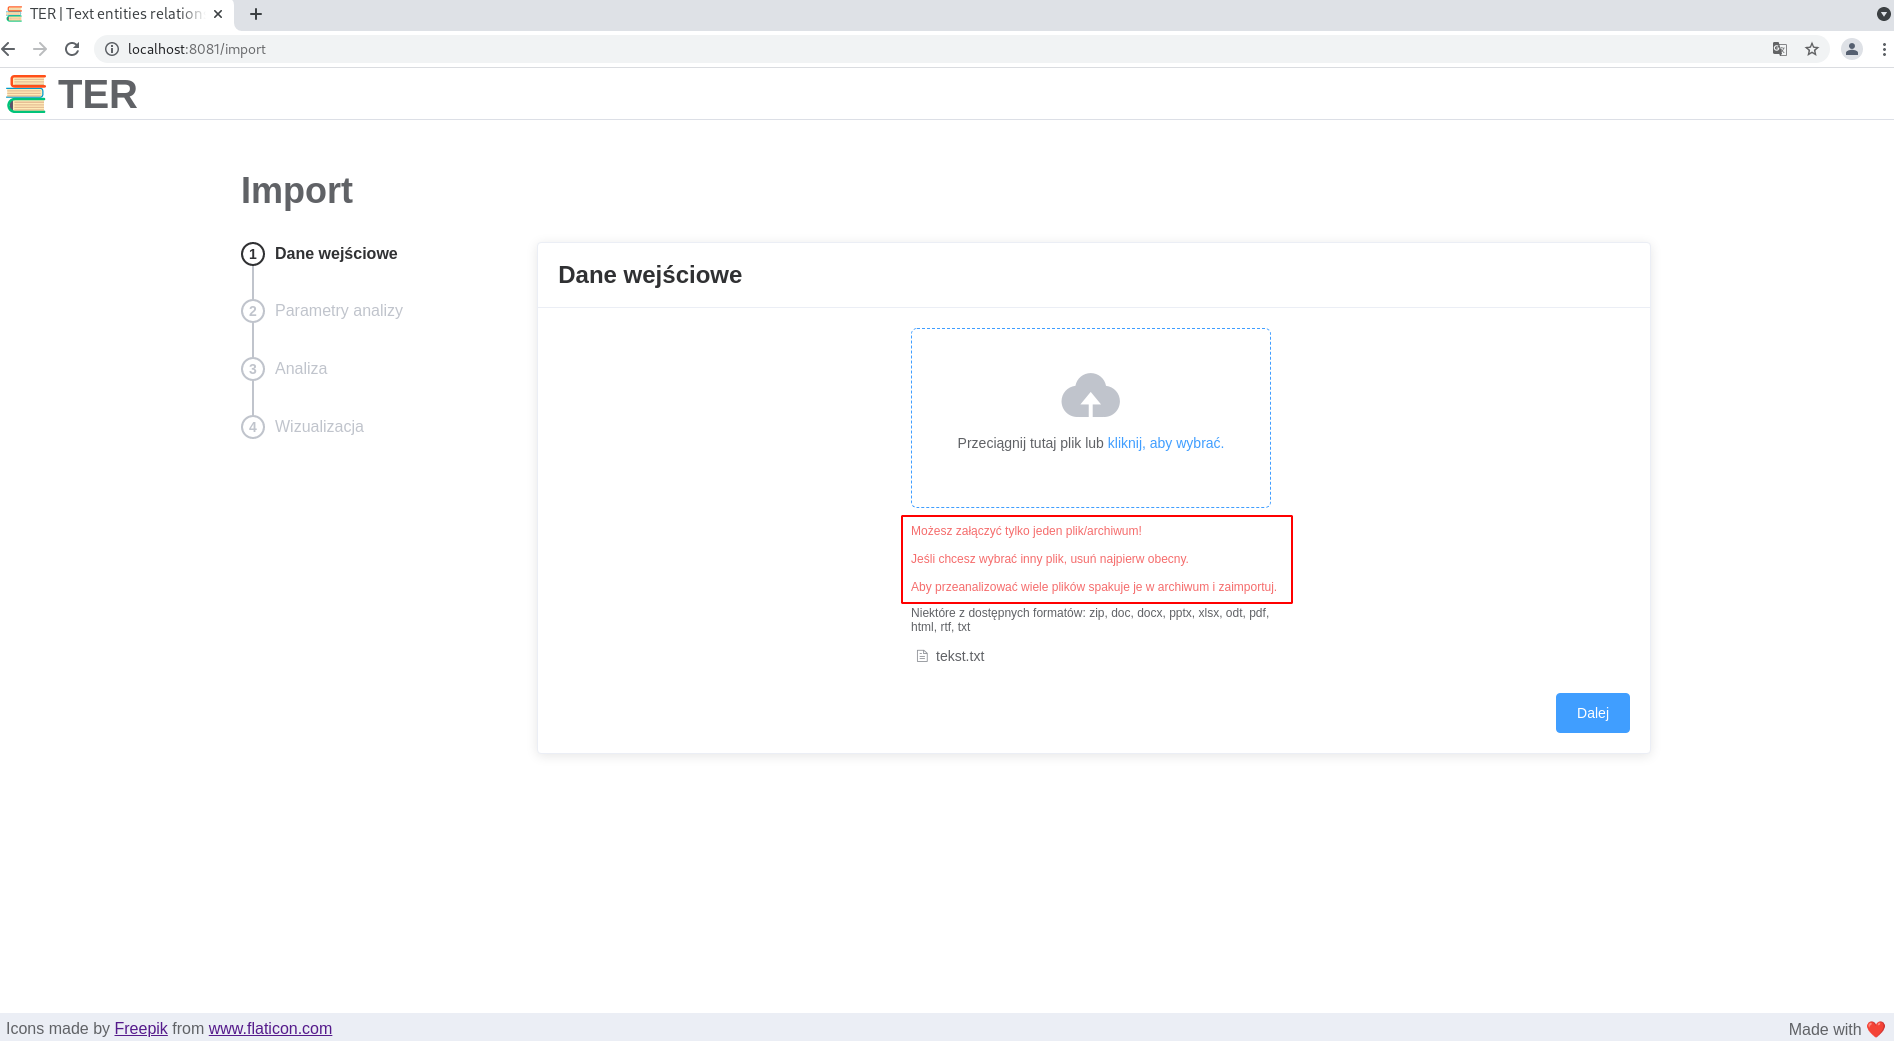
\includegraphics[width=\linewidth]{images/import-error.png}
  \caption{Przekroczenie limitu}
\end{figure}

Zgodnie z~informacją załączyć zawsze możemy \textit{jeden} plik lub archiwum. Jeśli chcemy dokonać analizy tekstów, które znajdują się w~różnych plikach, należy je wszystkie spakować do~archiwum o~rozszerzeniu zip i~zaimportować uzyskane archiwum do aplikacji. Oczywiście teksty nie muszą być spokrewnione lub~pochodzić od~jednego autora, narzędzie NER automatycznie dokona ekstrakcji tekstu z~przesłanych plików i~przeanalizuje dokument jako jedną całość. Dzięki temu możemy, przykładowo, odnaleźć powiązania między bohaterami z~różnych części sagi lub inne analogiczne relacje.

Jeśli popełniliśmy błąd i~chcemy wybrać inny plik do zaimportowania, należy najechać na~nazwę pliku, który już zaimportowaliśmy (na zrzucie ekranu \textit{szlengel-co-czytalem-umarlym.pdf}), po~czym ukaże nam się krzyżyk po prawej stronie, pozwalający na usunięcie pliku.

Wybierając przycisk \textit{Dalej}, który dostępny jest wyłącznie po~wcześniejszym zaimportowaniu pliku/archiwum przechodzimy do~ustalenia końcowych parametrów potrzebnych do~analizy.

\subsubsection{Parametry analizy}\label{parametry-analizy}

\begin{figure}[H]
  \centering
  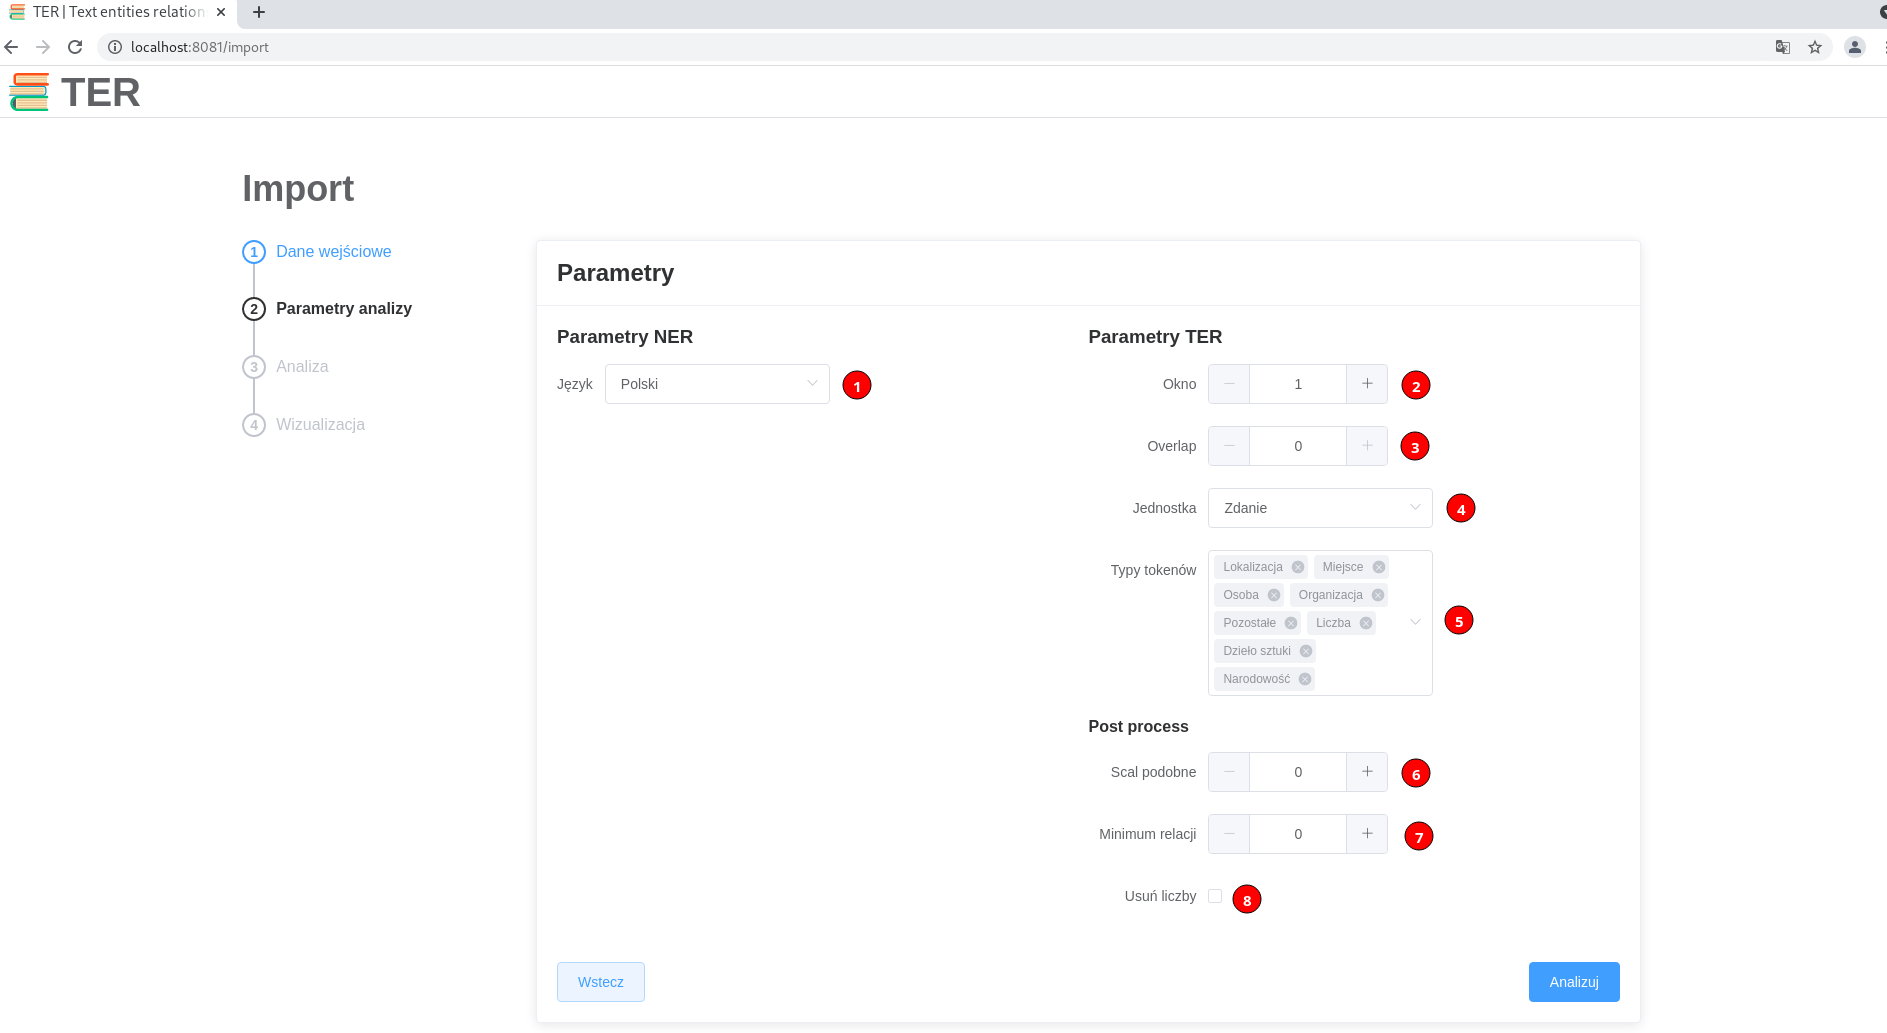
\includegraphics[width=\linewidth]{images/parameters.png}
  \caption{Wybór parametrów analizy}
\end{figure}

\noindent\textbf{Opcja 1, Język} -- Po naciśnięciu na~strzałkę ukazuje nam się lista z~obsługiwanymi językami. Wybieramy język w~jakim napisany jest zaimportowany wcześniej tekst.\\

\noindent\textbf{Opcja 2, Okno} -- ustalamy wartość okna, czyli zakresu w~jakim muszą pojawić się dwa znalezione byty, aby algorytm uznał, że są one w~relacji. Jak widzimy na zrzucie ekranu w~punkcie czwartym, w~polu jednostka ustawioną mamy wartość zdanie, oznacza to, że okno w~zaprezentowanym przykładzie stanowi $1$ zdanie, więc wszystkie słowa, które zostaną zidentyfikowane jako potencjalne byty i~\textit{występować będą w~obrębie jednego zdania}, zostaną połączone relacją. Jeśli ustawilibyśmy okno na~wartość $5$, a~w~polu jednostka wybralibyśmy wartość paragraf, oznaczałoby to, że~wyznaczamy relację spośród wszystkich słów, znajdujących się w~obrębie $5$ paragrafów w~tekście.\\

\noindent\textbf{Opcja 3, Overlap} -- Overlap jest parametrem, który wykorzystywany jest przez algorytm podczas wykrywania relacji między bytami. W~zaprezentowanym przykładzie wynosi on $0$, co oznacza, że podczas analizy nie wykryjemy żadnych relacji między bytami, które występują w~\textit{różnych} zdaniach (ponieważ jednostka ustawiona jest na wartość \textit{zdanie}, dla pozostałych wartości zachodzi analogiczna sytuacja). Parametr overlap pozwala nam określić ile jednostek (opcja numer 4) ma na siebie nachodzić podczas analizy. Dla przykładu jeśli ustalimy okno na wartość $5$, overlap na $2$, a~jednostkę stanowi zdanie, oznacza to, iż byty znalezione w~obrębie każdego okna składającego się z~$5$ zdań, gdzie każde $2$ ostatnie zdania jednego okna są pierwszymi dwoma zdaniami kolejnego, będą z~sobą w~relacji. Tak jak widzimy, parametr pozwala na rozwiązanie problemu analizy bytów wyłącznie w~obrębie pojedynczej jednostki wybranej w~opcji numer $4$.\\

\noindent\textbf{Opcja 4, Jednostka} -- Jednostka stanowi wartość, w~obrębie której chcemy wykrywać sąsiedztwo między znalezionymi wcześniej w~tekście bytami. Aby narzędzie NER poprawnie znajdowało paragrafy, powinny one być rodzielone co najmniej dwoma następującymi po~sobie w~tekście znakami nowej linii.\\

\noindent\textbf{Opcja 5, Typy tokenów} -- Narzędzie NER oprócz wykrywania bytów w~tekstach, dostarcza również informacji o~tym, do~jakiej kategorii konkretne wyrażenie zostało zaklasyfikowane. Klikając w~menu ukaże nam się lista z~wszystkimi dostępnymi typami bytów. Jeśli nie interesują nas jakieś typy jednostek, możemy je tutaj wykluczyć, dzięki czemu zostaną one pominięte podczas wyznaczania sąsiedztwa. Przykładowo, w~tekście może znajdować się wiele nazw lokalizacji, a~nas interesują głównie bohaterowie, więc możemy odfiltrować nazwy miejsc poprzez odznaczenie tej kategorii.\\

\noindent\textbf{Opcja 6, Scal podobne} -- Po najechaniu na opcję scalania ukaże nam się komunikat z~następującą informacją: ,,\textit{Scal wierzchołki, pomiędzy którymi odległość Levenshteina nie przekracza podanej liczby}''. Narzędzie lematyzujące używane przez serwis NER nie zawsze daje poprawny rezultat, co powoduje, że niektóre byty mogą wystąpić wielokrotnie w~różnych odmianach. W~związku z~tym opcja ta pozwala nam uniknąć wielu wierzchołków w~końcowym grafie, które w~rzeczywistości są na przykład tym samym bohaterem. Łączenie bytów odbywa się na bazie algorytmu Levenshteina, którego opis znaleźć można pod adresem \url{https://pl.wikipedia.org/wiki/Odleg\%C5\%82o\%C5\%9B\%C4\%87_Levenshteina}.\\

\noindent\textbf{Opcja 7, Minimum relacji} -- Po najechaniu na opcję, ukaże nam się komunikat z~następującą informacją: ,,\textit{Usuń wierzchołki, które mają mniej relacji niż podana liczba}''. Jeśli w~tekście występuje dużo bytów, które nie wchodzą w~relację z~innymi, może okazać się, że~graf będzie zawierał dużo nieistotnych obiektów, ponieważ przykładowo interesować będą nas tylko główni bohaterowie powieści. Opcja ta pozwala automatycznie pozbyć się bytów, które nie spełniają zadanego minimum, to znaczy, jeśli liczba ich relacji jest mniejsza od~ustalonej liczby, zostaną one pominięte w~końcowym grafie.\\

\noindent\textbf{Opcja 8, Usuń liczby} -- Zaznaczamy opcję jeśli nie chcemy podczas analizy brać pod~uwagę bytów, które są liczbami. Jest to opcja analogiczna do~usunięcia tokenów o~typie liczba w~opcji numer $5$, lecz narzędzie NER nie zawsze kategoryzuje poprawnie rozpoznawane byty, w~związku z~czym opcja ta powinna poprawić końcowy rezultat.\\

Po zakończonej konfiguracji wybieramy przycisk Analizuj, który przeniesie nas na następny widok i~automatycznie rozpocznie analizę tekstu na podstawie skonfigurowanych parametrów.


\subsubsection{Analiza}

\begin{figure}[H]
  \centering
  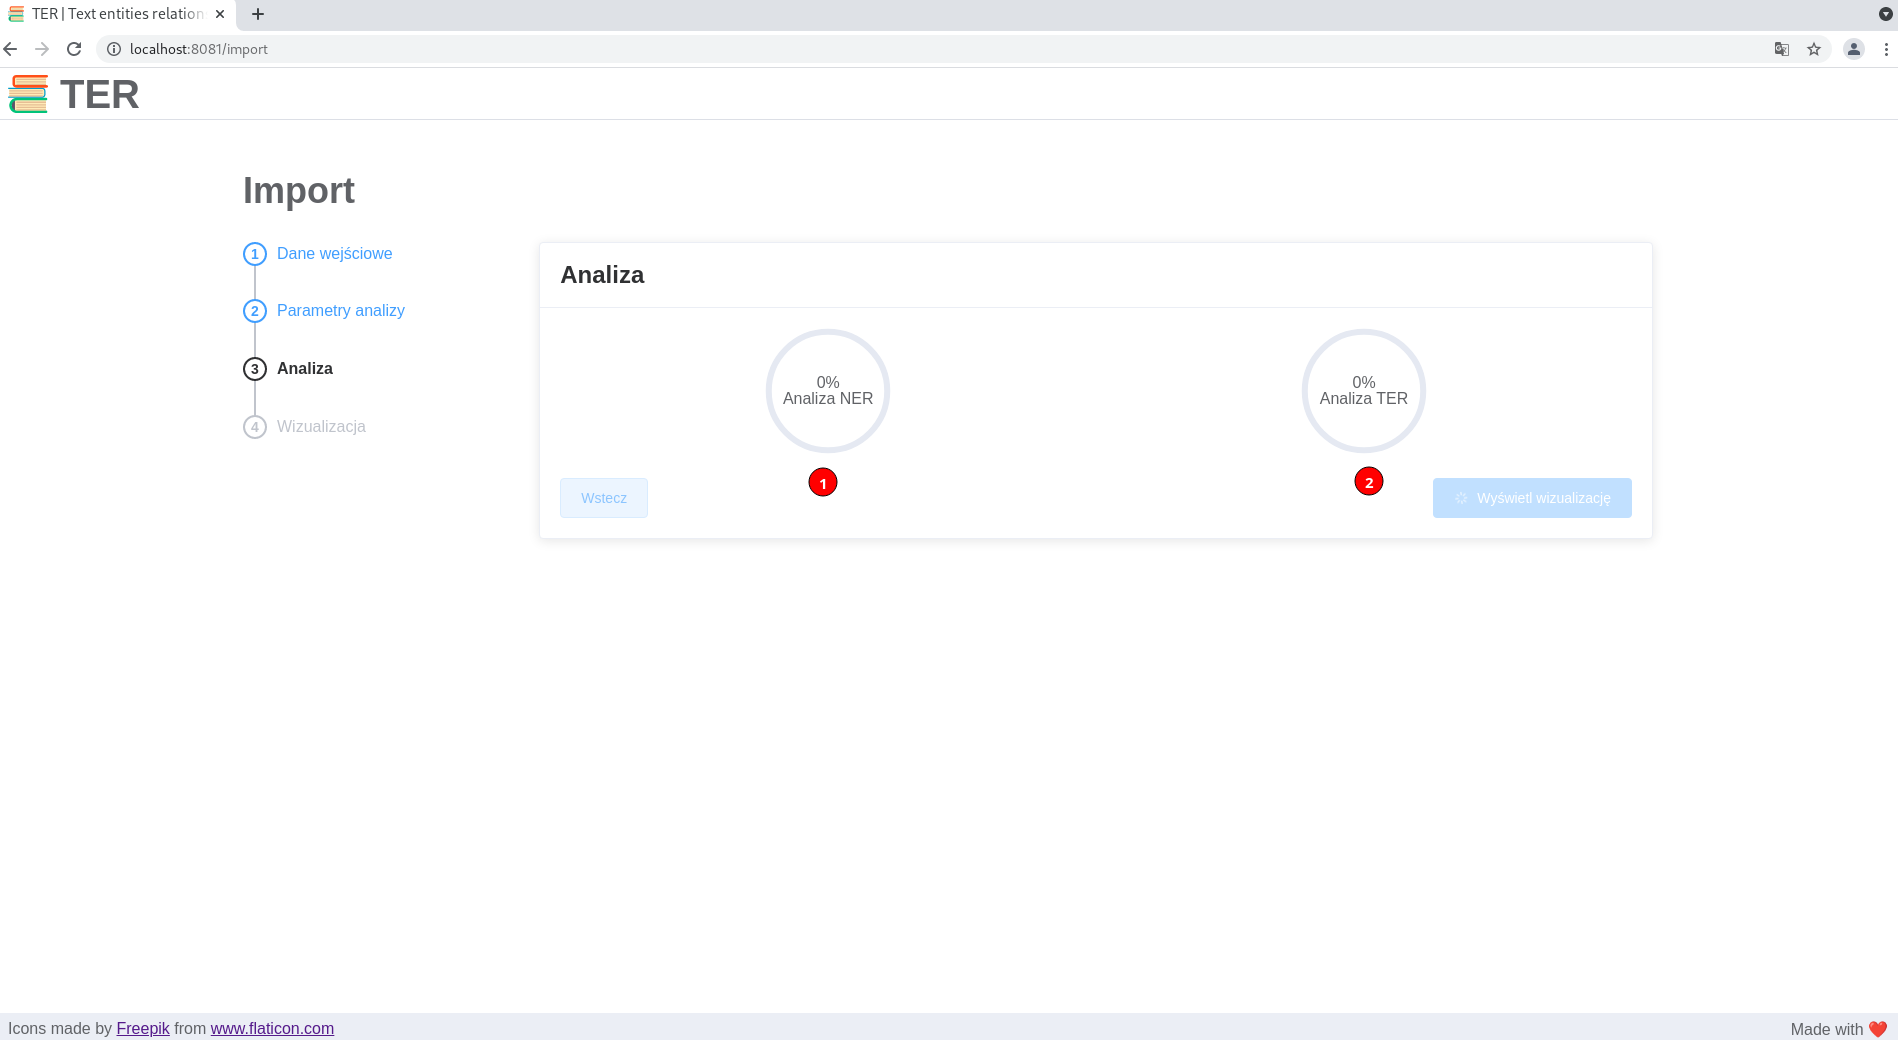
\includegraphics[width=\linewidth]{images/analiza.png}
  \caption{Widok analizy}
\end{figure}

Na tym widoku możemy na bieżąco śledzić postęp analizowanego pliku. Tak długo jak analiza jest w~trakcie wykonywania oba przyciski są niedostępne.\\

\noindent\textbf{Postęp 1, Analiza NER} -- Okrąg informuje nas o~postępie w~analizie pliku przez~zewnętrzny serwis NER, który dokonuje identyfikacji bytów na bazie przekazanych przez nas parametrów oraz próbuje dokonać ich lematyzacji. Należy pamiętać, że serwis ten może być wykorzystywany przez wiele osób jednocześnie w~związku z~czym nasz plik może nie zostać przeanalizowany natychmiastowo i~trafi do~kolejki. W~takim wypadku nie należy zamykać strony, tylko zaczekać do~czasu zakończenia analizy.\\

\noindent\textbf{Postęp 2, Analiza TER} -- Okrąg informuje nas o~postępie wykrywania sąsiedztwa pomiędzy zidentyfikowanymi przez serwis NER bytami.

\begin{figure}[H]
  \centering
  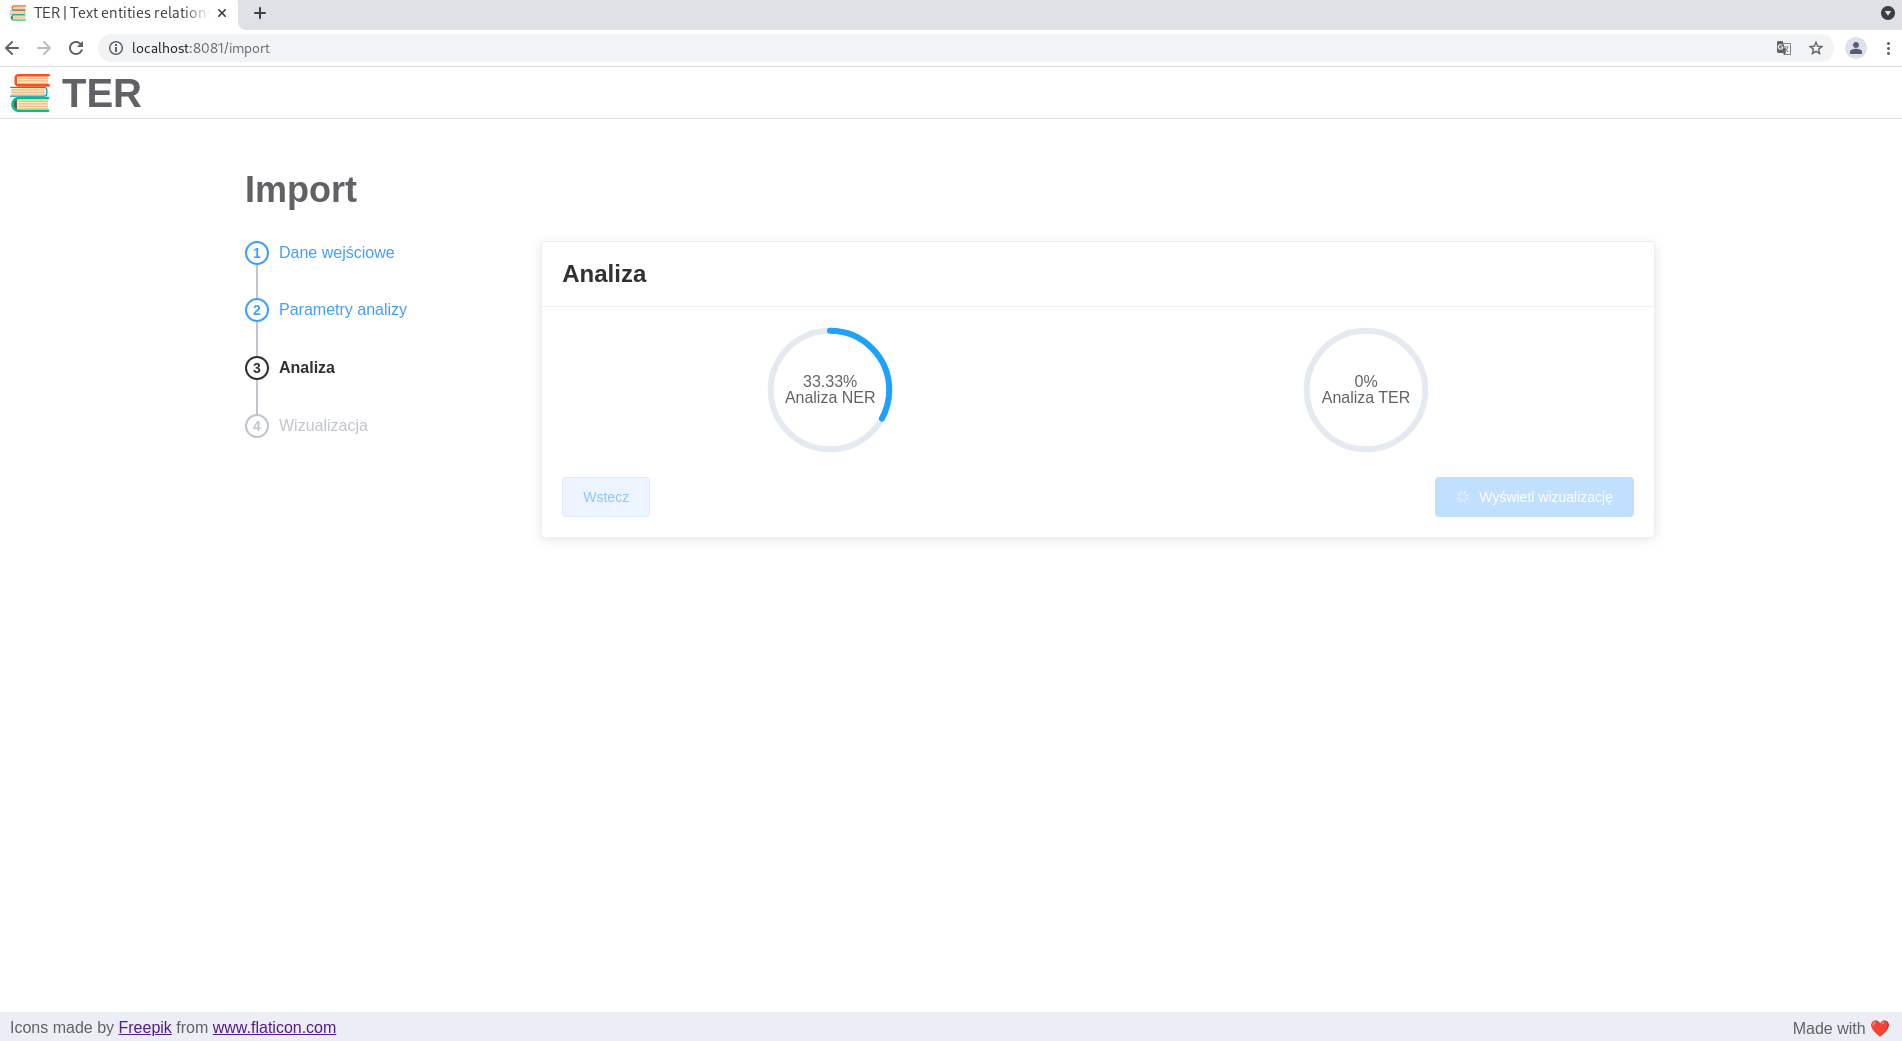
\includegraphics[width=\linewidth]{images/analiza-w-trakcie.png}
  \caption{Postęp w~analizie}
\end{figure}

Jeśli podczas analizy dojdzie do błędu, adekwatny komunikat zostanie wyświetlony na ekranie. w~takim wypadku, należy skontaktować się z~administratorem aplikacji i~mieć przygotowany problematyczny plik. Istnieje również możliwość, że serwis NER jest czasowo niedostępny w~związku z~czym należy spróbować zaimportować plik później.

\begin{figure}[H]
  \centering
  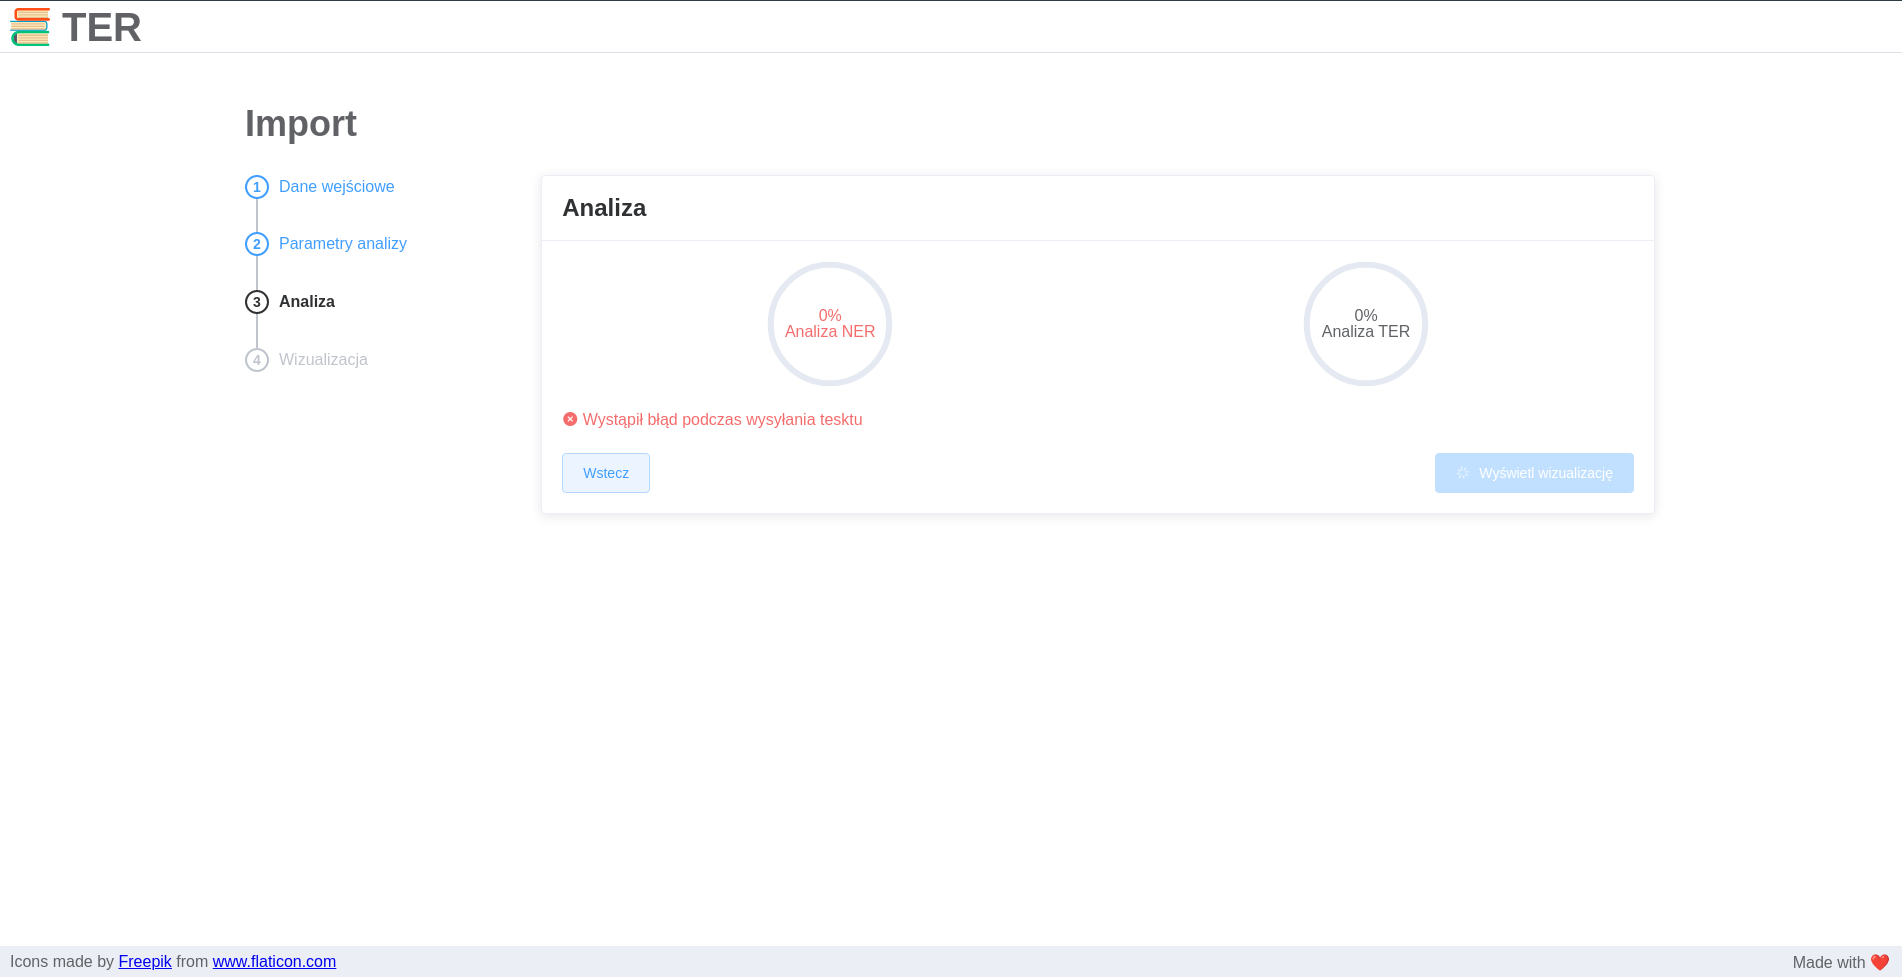
\includegraphics[width=\linewidth]{images/analiza-error.png}
  \caption{Błąd podczas analizy}
\end{figure}

Po~poprawnie zakończonej analizie, przy~pomocy przycisku wyświetl wizualizację, należy przejść do~widoku z~grafem, który pozwala nam na interakcję z~odnalezionymi bytami.

\begin{figure}[H]
  \centering
  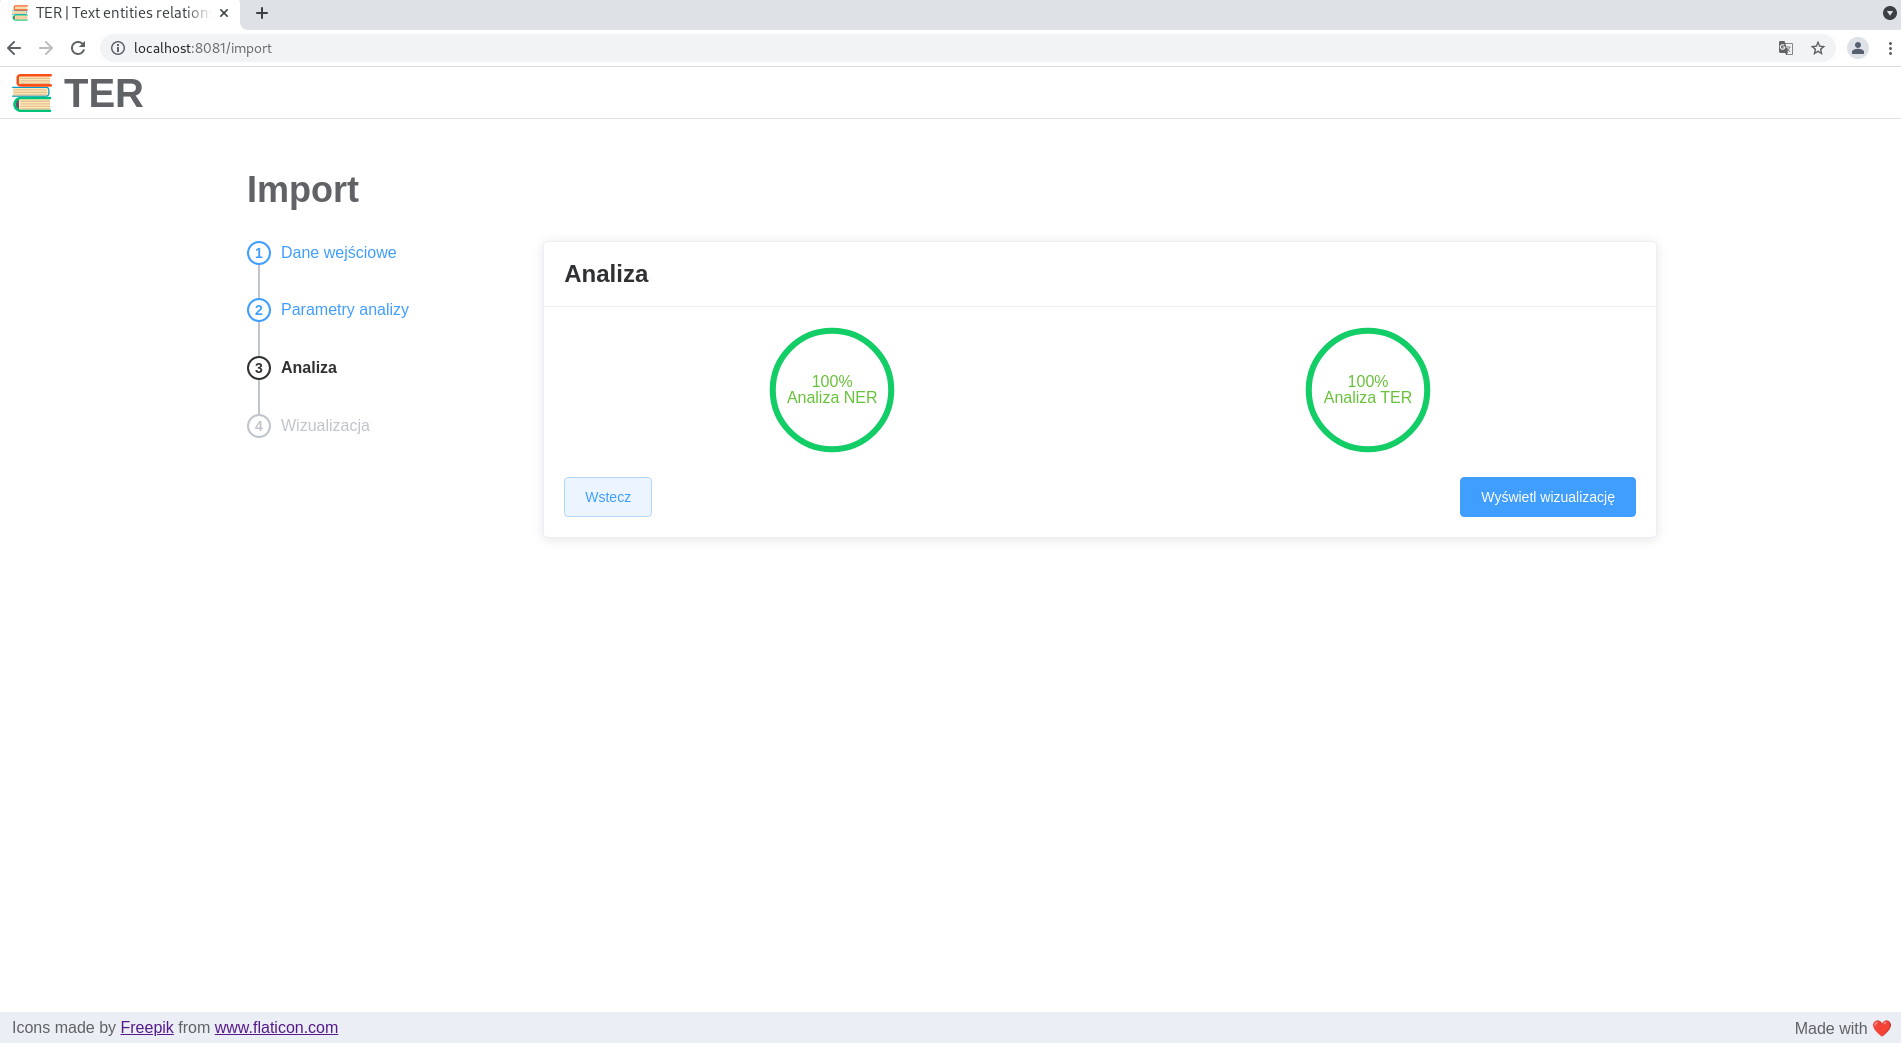
\includegraphics[width=\linewidth]{images/analiza-success.png}
  \caption{Poprawnie zakończona analiza}
\end{figure}

\subsection{Widok grafu prezentującego wizualizację}\label{section:graph}

Przedstawiony poniżej graf jest wynikiem wcześniej przeprowadzonej analizy (z dokładnie takimi samymi parametrami jak na wcześniejszych zrzutach ekranu) na opowiadaniu pod tytułem ,,\textit{Co czytałem umarłym}''.

\begin{figure}[H]
  \centering
  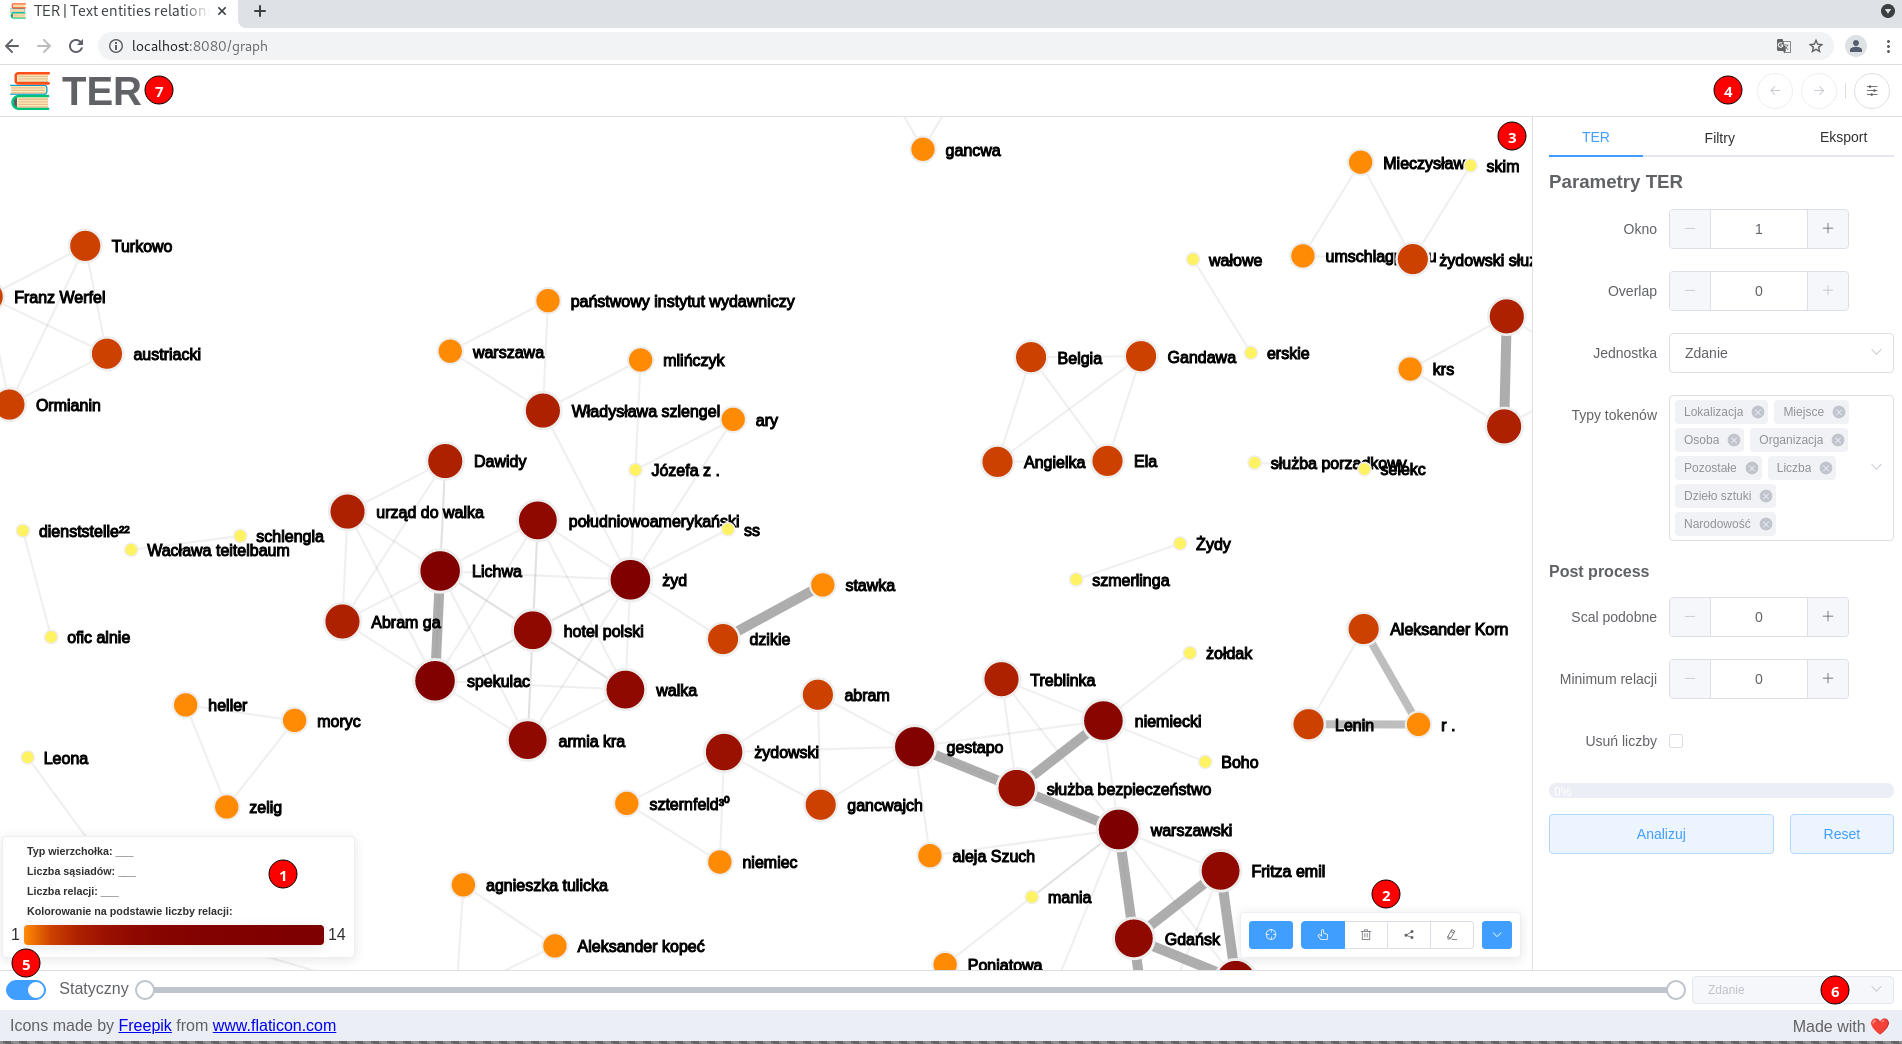
\includegraphics[width=\linewidth]{images/graf-main.png}
  \caption{Początkowy widok grafu}
  \label{graf-main}
\end{figure}

Jak widzimy na~zrzucie \ref{graf-main}, po~poprawnie zakończonej analizie we~wcześniejszych krokach uzyskujemy graf, w~którym byty z~największą ilością relacji mają odpowiednio ciemniejszą barwę oraz~są większe od~pozostałych zidentyfikowanych encji. Dodatkowo, połączenia pomiędzy bytami mają różną grubość i~widoczność, które zależne są od~siły danej relacji, czyli tego jak często pojawiła się ona w~przeanalizowanym tekście.\\

\subsubsection{Szczegóły wierzchołka, 1}

Po najechaniu na~wybrany wierzchołek uzyskujemy dodatkowe informacje na~jego temat. Przykładowo najeżdżając na~wierzchołek o~nazwie \textit{gestapo} ukazuje nam się poniższy wynik.

\begin{figure}[H]
  \centering
  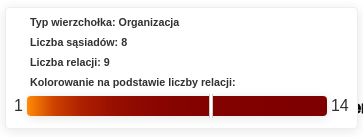
\includegraphics[width=0.6\linewidth]{images/graph-gestapo.png}
  \caption{Szczegóły wierzchołka \textit{gestapo}}
\end{figure}

\noindent\textbf{Typ wierzchołka} określany jest przez serwis NER i~ze~względu na~trudność w~identyfikacji poszczególnych bytów, wartość ta może być nieprawidłowa.\\\\
\textbf{Liczba sąsiadów} stanowi liczbę bytów, która jest w~relacji z~obserwowanym przez nas wierzchołku.\\\\
\textbf{Liczba relacji} natomiast mówi o~tym, ile razy relacje pojawiły się w~tekście. Jeśli liczba relacji jest większa od~liczby sąsiadów oznacza to, że niektóre z~tych relacji musiały pojawić się kilka razy w~tekście. Dla podanego przykładu możemy zauważyć, że relacja między bytami \textit{gestapo} i~\textit{warszawski} wystąpiła częściej niż pozostałe, ponieważ na~grafie połączenie to jest znacznie grubsze.\\\\
\textbf{Kolorowanie na podstawie liczby relacji} jest graficzną reprezentacją liczby relacji. Przedział dla przykładowego grafu wynosi od $1$ do $14$ co oznacza, że dane byty w~przeanalizowanym tekście miały od $1$ do $14$ relacji.

\subsubsection{Poruszanie się po grafie, 2}\label{graph-movement}

Domyślnie po~inicjalizacji grafu, automatycznie wybrana zostaje opcja, przeciągania wierzchołków w~dowolny punkt. Dodatkowo zaimplementowano możliwość przybliżania i~oddalania całego widoku przy~pomocy kółka myszy. Podwójne kliknięcie w~miejsce w~którym \textit{nie} znajduje się żaden wierzchołek, spowoduje przybliżenie wybranej części grafu.

\begin{figure}[H]
  \centering
  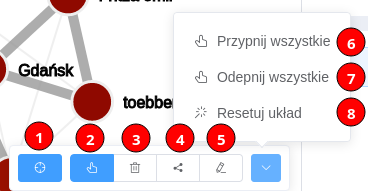
\includegraphics[width=0.6\linewidth]{images/graph-menu.png}
  \caption{Menu grafu}
  \label{graph-menu}
\end{figure}

\noindent \textbf{Opcja 1, wyśrodkuj} -- Po~naciśnięciu pozwala nam dopasować obecny wygląd grafu do~szerokości okna przeglądarki. Zalecane jest, aby użyć tej funkcji po~inicjalizacji grafu, ponieważ wyśrodkuje ona cały układ i~pozwoli dokładnie zobaczyć całość. Funkcję można też wykorzystywać, kiedy chcemy szybko dopasować widok do położenia wszystkich wierzchołków.\\

\noindent \textbf{Opcja 2, przypnij} -- Wierzchołki grafu domyślnie są nieprzypięte, dzięki czemu rozkładają się tak, aby całość była czytelna i~po przeciągnięciu w~dowolne miejsce starają się wrócić do swoich sąsiadów. Jeśli będziemy mieli zaznaczoną opcję numer $2$ (tak jak na zrzucie ekranu, zaznaczenie określane jest poprzez podświetlenie na niebiesko wybranej opcji), w~momencie przeciągnięcia wierzchołka zostaje on przypięty i~nie będzie się on już poruszał. Aby odpiąć wierzchołek należy kliknąć na niego dwukrotnie.\\

\noindent \textbf{Opcja 3, usuń} -- Po wybraniu opcji, kliknięcie na wierzchołek usuwa go z~grafu i~automatycznie przelicza wszystkie pozostałe relacje, tak aby poprawnie zaktualizować stan grafu.\\

\noindent \textbf{Opcja 4, scal} -- Jeśli w~grafie znajdują się wierzchołki, które zostały zidentyfikowane jako osobne byty, a~w~rzeczywistości są one na przykład jednym bohaterem, po wybraniu tej opcji możemy przy pomocy klikania na odpowiednie wierzchołki scalić je w~jeden, dzięki czemu relacje zostaną odpowiednio zaktualizowane tak aby usunąć potencjalny szum z~grafu.

Proces scalania obejmuje zawsze dwa wierzchołki i~polega na scaleniu pierwszego wybranego wierzchołka z~kolejnym wybranym. Aby ułatwić ten proces, po wybraniu opcji numer $4$ i~kliknięciu w~wybrany wierzchołek pokazuje nam się animacja, która prezentuje byt do~którego będziemy scalać nasz kolejny wybór. w~uzyskanym grafie widzimy, że zidentyfikowane zostały byty \textit{żyd} i~\textit{żydowski}, które w~rzeczywistości reprezentują tę samą encję. W~celu scalenia, wybieramy opcję numer $4$ i~następnie klikamy na wierzchołek \textit{żyd}, co powoduje jego podświetlenie.

\begin{figure}[H]
  \centering
  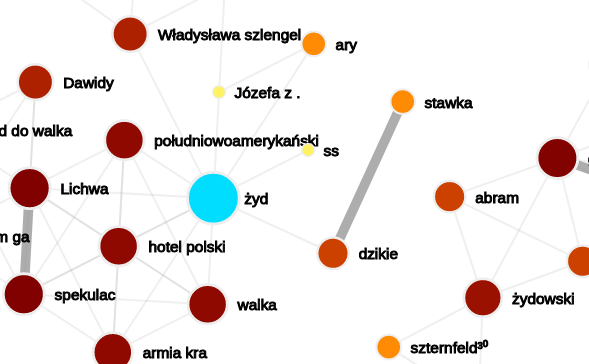
\includegraphics[width=0.7\linewidth]{images/graph-jew-highlight.png}
  \caption{Podświetlony wierzchołek \textit{żyd}}
\end{figure}

Następnie klikamy w~wierzchołek \textit{żydowski} i~widzimy jak automatycznie relacje z~bytu \textit{żydowski} zostały przepięte do wierzchołka \textit{żyd}.

Jeśli pomyliliśmy się przy zaznaczaniu wierzchołka, możemy na niego kliknąć ponownie lub nacisnąć klawisz \textit{ESC}, aby go odznaczyć. Aby ułatwić dalszy proces scalania wierzchołków zaimplementowano możliwość zaznaczania wierzchołka z~przytrzymanym klawiszem \textit{Shift}, dzięki czemu po pierwszej operacji scalenia, nasz bazowy wierzchołek jest ciągle zaznaczony i~możemy od razu przejść do połączenia kolejnych wierzchołków.\\

\noindent \textbf{Opcja 5, zmień nazwę} -- Część bytów może mieć źle odmienione, bądź w inny sposób niepoprawne nazwy. Po wybraniu tej opcji i~naciśnięciu na interesujący nas wierzchołek, ukazuje nam się animacja oraz okno dialogowe w~którym możemy nadać nową nazwę encji. Przykładowo, w~naszym grafie widzimy encję o nazwie \textit{ul .} i~chcielibyśmy aby wierzchołek ten nazywał się \textit{ulica}. Wybieramy więc opcję numer $5$, wpisujemy nową nazwę i~zatwierdzamy wybór strzałką z~prawej strony jak na~zrzucie ekranu poniżej.

\begin{figure}[H]
  \centering
  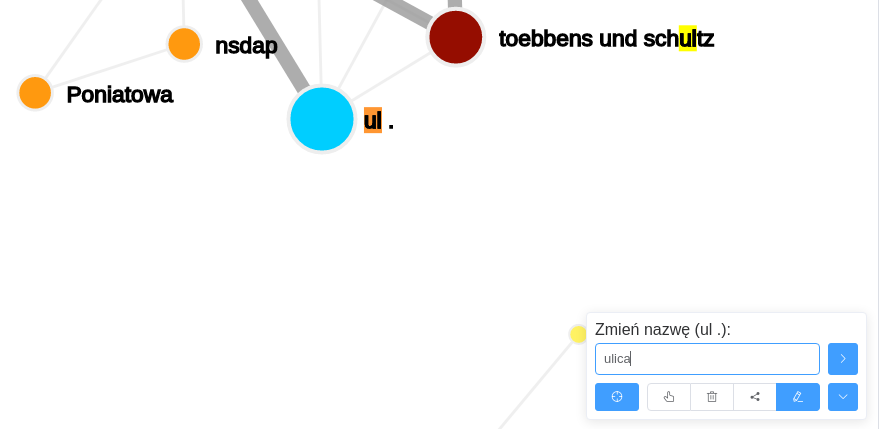
\includegraphics[width=0.7\linewidth]{images/graph-ulica.png}
  \caption{Zmiana nazwy wierzchołka \textit{ul .}}
\end{figure}

Oczywiście może dojść do sytuacji, w~której zmienimy nazwę wierzchołka na taką, która już obecnie występuje w~grafie, w~takiej sytuacji aplikacja zapyta nas, czy chcemy dokonać automatycznego scalenia wierzchołków i~jeśli potwierdzimy nasz wybór, całość zakończy się poprawnie. Przykładowo, jeśli spróbujemy zmienić nazwę wierzchołka \textit{heller} na~\textit{Heller} pojawi nam się stosowny komunikat. Wybranie przycisku tak dokona automatycznego scalenia.

\begin{figure}[H]
  \centering
  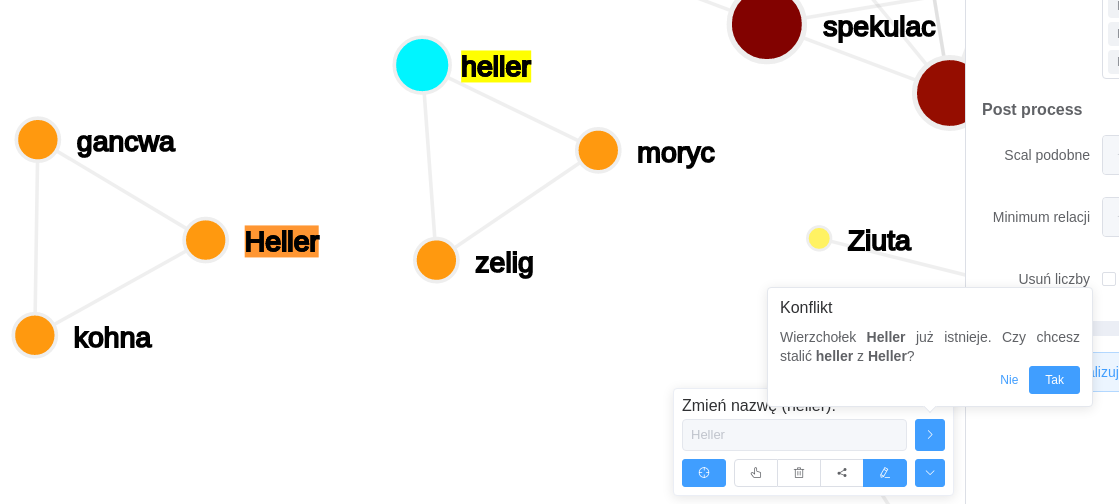
\includegraphics[width=0.7\linewidth]{images/graph-change-name-heller.png}
  \caption{Zmiana nazwy wierzchołka \textit{heller}}
\end{figure}


\noindent \textbf{Opcja 6, przypnij wszystkie} -- Jeśli chcemy szybko unieruchomić obecny stan grafu, po~najechaniu na strzałkę w~prawym dolnym rogu menu z~zrzutu ekranu \ref{graph-menu} ukazują nam się dodatkowe opcje i~pierwsza z~nich pozwala zablokować cały układ. Opcja przydaje się podczas pracy na grafie, ponieważ wierzchołki po usunięciu lub scaleniu nie~będą wtedy się przemieszczały, dążąc do~zbliżenia się do swoich sąsiadów.\\

\noindent \textbf{Opcja 7, odepnij wszystkie} -- Jest to funkcjonalność przeciwna do tej z~poprzedniego punktu, pozwalająca na~ożywienie całego układu i~spowodowania wzajemnego przyciągania wierzchołków.

\noindent \textbf{Opcja 8, resetuj układ} -- Jeśli dokonaliśmy wielu modyfikacji, nasz graf uległ znacznemu zniekształceniu i~chcielibyśmy zresetować jego układ (bez modyfikacji danych), wybieramy tę opcję, dzięki czemu wierzchołki rozłożą się od nowa.

\subsubsection{Zakładka boczna, 3}

W~tej zakładce zostały umieszczone wszystkie pozostałe operacje, które możemy realizować z~poziomu grafu.

\subsubsubsection{Zakładka TER}

\begin{figure}[H]
  \centering
  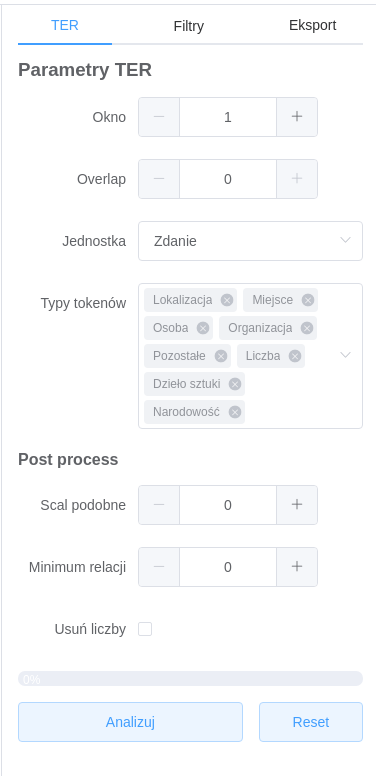
\includegraphics[width=0.4\linewidth]{images/graph-ter.png}
\end{figure}

Jest to widok, który znamy już z~sekcji \ref{parametry-analizy} i~oferuje on dokładnie te same możliwości, które zostały dokładnie opisane wcześniej. Funkcja ta pozwala szybko ponowić analizę \textit{TER} a~więc tylko część odpowiedzialną za~wykrywanie relacji między bytami a~nie~ich identyfikację w~tekście przy~pomocy serwisu NER. Jest to przydatne narzędzie, gdy uzyskany przez~nas początkowy graf nas nie satysfakcjonuje, dokonaliśmy błędnego wyboru parametrów lub~zapomnieliśmy zaznaczyć pewnych opcji. Należy pamiętać, że ponowna analiza \textbf{usunie dokonane przez~nas dotychczas zmiany} o czym zostaniemy poinformowani w~stosownym komunikacie, przedstawionym poniżej.

\begin{figure}[H]
  \centering
  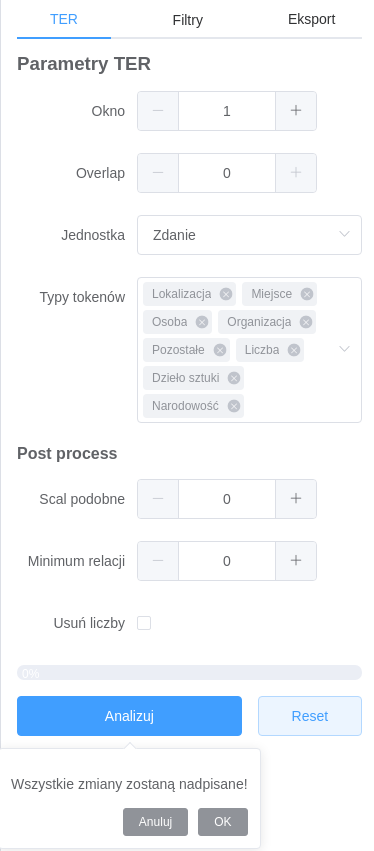
\includegraphics[width=0.4\linewidth]{images/graph-ter-erase.png}
\end{figure}

\subsubsubsection{Zakładka Filtry}

Widok ten pozwala nam dynamicznie filtrować wierzchołki o interesujących nas nazwach i~właściwościach.

\begin{figure}[H]
  \centering
  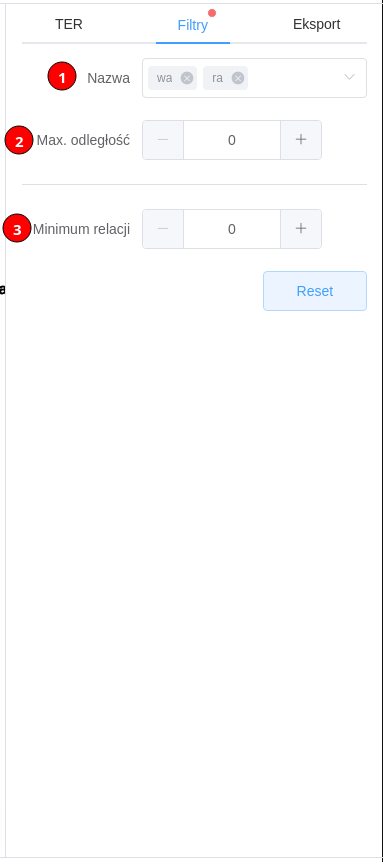
\includegraphics[width=0.4\linewidth, trim={0 14cm 0.2cm 0},clip]{images/graph-filters.png}
\end{figure}

\noindent \textbf{Opcja 1, Nazwa} --  Filtr został zbudowany w~taki sposób, że możemy wpisywać wiele fraz i~wyświetlone zostaną wierzchołki, których nazwy zawierają filtrowane frazy.\\

\noindent \textbf{Opcja 2, Max. odległość} -- Po najechaniu na~opcję ukazuje nam się komunikat \textit{Pokaż wierzchołki, które zawierają podane ciągi znaków, których odległość Levenshteina pomiędzy nazwą wierzchołka nie~przekracza podanej liczby.} Jest to uzupełnienie opcji numer~$1$ o~rozszerzenie filtracji, nie~tylko po~dokładnie zadanych nazwach, ale~również bliskich pod~względem odległości Levenshteina.\\

\noindent \textbf{Opcja 3, Minimum relacji} -- Chcemy zobaczyć wyłącznie wierzchołki, które mają większą od podanej liczbę relacji.

\subsubsubsection{Zakładka Export}

Ostatnia zakładka pozwala na~wyeksportowanie obecnego stanu grafu do~jednego z~trzech formatów:

\begin{enumerate}
  \item \textbf{TER} -- jest to format pliku używany wyłącznie przez tę aplikację. Plik ten można wczytać na ekranie startowym aplikacji przedstawionym na~zrzucie \ref{main-view}, tak aby od~razu przejść do~widoku grafu i~pominąć analizę. Format ten jest najprostszym sposobem podzielenia się wynikiem pracy z~innymi osobami, które również chciałyby pracować z~aplikacją.
  \item \textbf{GEPHI} -- możliwość wyeksportowania efektu pracy do~popularnego sposobu reprezentacji grafów przy~pomocy formatu XML. Plik ten może zostać później wczytany do~wybranego narzędzia obsługującego taki format.
  \item \textbf{CSV} -- Plik tekstowy w~którym zawarte są wszystkie dane odnośnie wierzchołków oraz~ich relacji. Przydatny do~dalszej pracy w oprogramowaniu do~arkuszów kalkulacyjnych (np. MS~Excel), bądź do~programowego przetwarzania danych (np. skrypt w~Python).
\end{enumerate}

\begin{figure}[H]
  \centering
  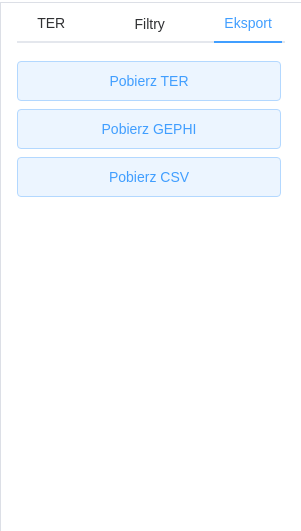
\includegraphics[width=0.4\linewidth, trim={0 8cm 0 0},clip]{images/graph-export.png}
\end{figure}

\subsubsection{Górna nawigacja, 4}

Ta część interfejsu pozwala nam korygować nasze błędy oraz~przywracać wcześniejsze modyfikacje. Po~dokonaniu operacji usunięcia wierzchołka lub scalenia go z~innym, zawsze mamy możliwość cofnięcia się do~poprzedniego stanu grafu. Opcja ta aktywuje się wyłącznie po~dokonaniu modyfikacji, przykładowo po~operacji scalenia i~usunięcia wierzchołków z~poprzednich kroków możemy zauważyć zmianę w~interfejsie pokazaną poniżej.

\begin{figure}[H]
  \centering
  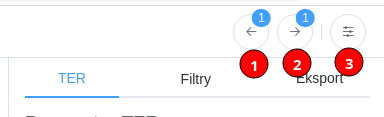
\includegraphics[width=0.6\linewidth]{images/graph-top-navigation.png}
  \caption{Historia operacji}
\end{figure}

\noindent Niebieskie dymki mówią nam o~tym, ile akcji możemy cofnąć lub~przywrócić. Funkcjonalność ta jest analogiczna do~tej dostępnej np. w programie MS~Word, gdzie cofamy, bądź przywracamy dokonane przez nas operacje. Dodatkowo opcja numer $3$ pozwala całkowicie schować boczny panel tak aby graf zajął całe dostępne w~oknie przeglądarki miejsce (warto wtedy ponownie wyśrodkować graf, tak aby dostosował się on do~nowego, większego ekranu).

\subsubsection{Dynamiczna wizualizacja, opcje 5 i~6}

Przełącznik w~dolnej części interfejsu pozwala odblokować możliwość przeglądania grafu w~czasie, to znaczy pomiędzy wybranymi zakresami zdań/słów/paragrafów, które konfigurujemy w~opcji numer $6$.

\begin{figure}[H]
  \centering
  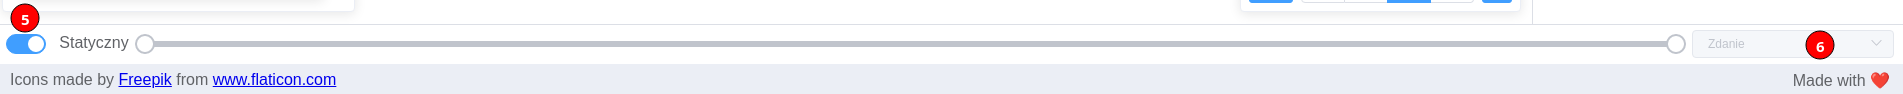
\includegraphics[width=\linewidth]{images/graph-down-menu.png}
  \caption{Opcja dynamicznego grafu}
\end{figure}

Gdy naciśniemy na~przełącznik numer $5$, odblokowany zostanie pasek z~prawej strony, na~którym zobaczymy zakres w~którym możemy się poruszać, wraz z~wyborem jednostki. Po~najechaniu na~końce zakończone okręgami zobaczymy numer, który mówi o~tym od~jakiego zdania/słowa/paragrafu obecnie widzimy byty i~ich relacje. Przykładowo, jeśli chcemy zobaczyć jakie byty zostały znalezione od $20$ do~$40$ paragrafu naszego opowiadania, wybieramy w~opcji numer $6$ jednostkę paragraf i~następnie adekwatnie przesuwany zakres na suwaku, tak jak na~zrzucie poniżej.

\begin{figure}[H]
  \centering
  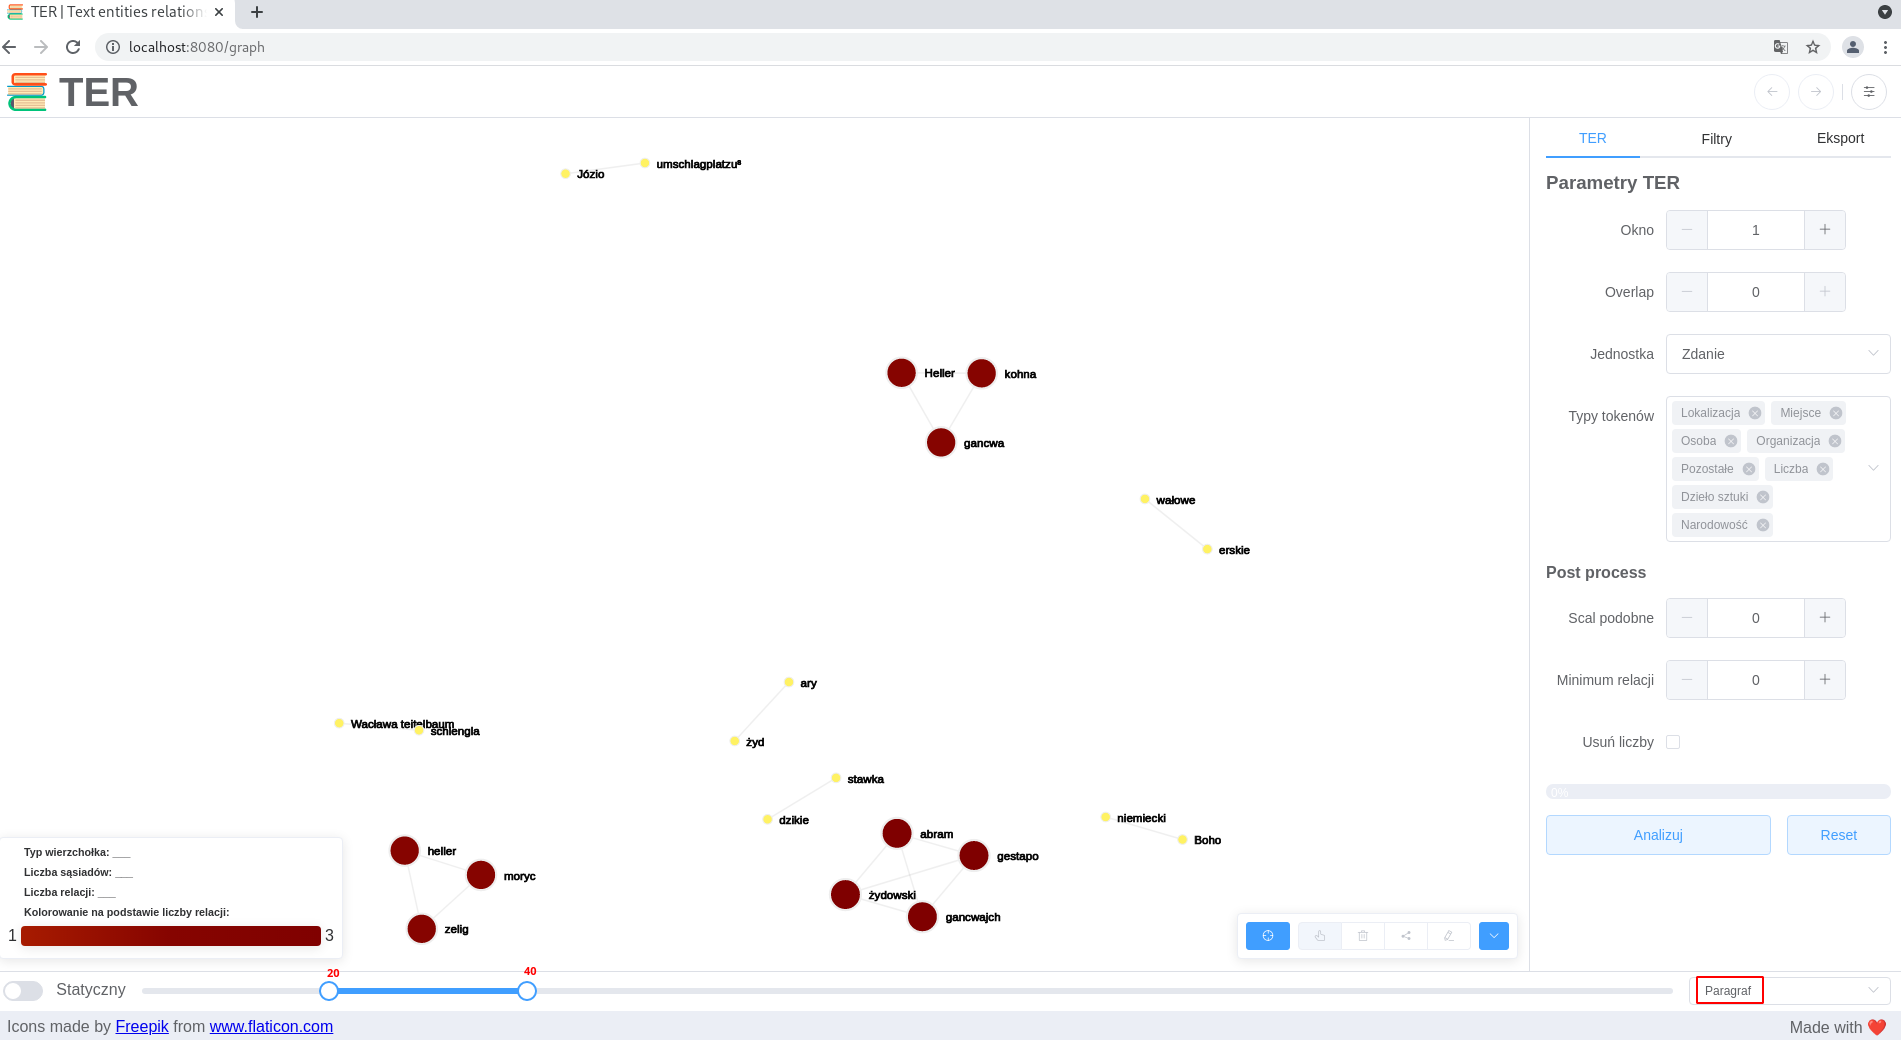
\includegraphics[width=\linewidth]{images/graph-dynamic.png}
  \caption{Wynik wizualizacji dynamicznej}
\end{figure}

Jak widzimy, opcja ta jest przydatna, gdy chcemy wizualizować sposób, w~jaki dochodziło do~interakcji między danymi bytami na~przestrzeni konkretnych miejsc w~analizowanym tekście. Opcja modyfikacji grafu na~widoku dynamicznym jest \textbf{wyłączona}, ponieważ każda zmiana w~danych grafu wpływała by na~wierzchołki i~relacje, które mogą nie~być aktualnie widoczne ze~względu na~dobrany zakres. Niemniej jednak na~grafie dynamicznym, możemy dokonywać wszystkich operacji związanych z~wizualizacją układu, w~tym między innymi zresetowania układu, tak jak opisano to wcześniej w~sekcji \ref{graph-movement} oraz~przypinania czy odpinania wierzchołków.

\subsubsection{Powrót do startowego widoku aplikacji, 7}

Górne logo pozwala nam w~prosty sposób wrócić do~widoku, od~którego rozpoczęliśmy pracę z~aplikacją. Załączone do~instrukcji pliki \textit{szlengel-co-czytalem-umarlym.pdf} oraz~\textit{co-czytalem-umarlym.ter} mogą zostać bezpośrednio wczytane do~aplikacji, tak aby móc dokładnie śledzić całą instrukcję.


%--/Paper--

\end{document}